\chapter{Overall Description}
\section{Product perspective}
In the section is presented a list of real sceanarios and diagrams illustrating further details about shared phenomenas.
\subsection{Scenarios}
\subsubsection{\nth{1} scenario: An end user needs to charge his vehicle}
Bob, who owns an electric vehicle and who previously registered to the system, while on the road needs to charge it. For this reason he opens the eMall app which offers him the charging stations closest to him, available at that precise moment with the relative charge prices and any offer available. Subsequently, he books, in that station, the desired socket for a certain time receiving a QR-Code to be shown at the socket scanner at the moment of charging. At the end of the process, the system notifies Bob of the end and automatically subtracts the cost of the charge and, moreover, it sends the invoice at the user's email address.
\subsubsection{\nth{2} scenario: An end user needs to delete a booking}
Bob is at home planning a trip, so he decides to look at the charging stations on his way by booking them in advance. During the booking, he realizes that he has mistakenly selected an unwanted station; for this reason, he deletes the booking using the appropriate section of the application.
\subsubsection{\nth{3} scenario: A CPO monitors a charging process}
Bob has started the charging process in a station at the rapid socket 3. Bob wants a coffee, so he goes to a nearby cafe, meanwhile the CPO can monitor, through the CPMS, the charging process of Bob's brand new car to check that everything is fine.
\subsubsection{\nth{4} scenario: A CPO installs a new charging station}
A CPO has just installed a new charging station that must be added to the system. So, through the CPMS the CPO can insert the new charging station providing specific information, i.e. number and type of each charging socket, coordinates, etc.
\subsubsection{\nth{5} scenario: A CPO makes an energy purchase}
\label{sec:explsaving}
A CPO wants to purchase energy from the most convenient DSO, choosing between different options presented by the system in order to provide end users with more and more appealing offers. Furthermore, since the price of energy today is lower than usual, the CPO decides to store the energy inside the batteries to maximize the profits as much as possible instead of acquiring energy directly from DSO.
\subsection{Class diagram}
Class diagrams are useful for illustrating relationship between classes and interfaces.
\begin{itemize}
    \item \textbf{User}: in eMall system, user is the general term to indicate \textbf{CPO} or \textbf{End user}.
    \item \textbf{End user}: represents an end user of eMSP software.
    \item \textbf{CPO}: represents a user of CPMS software.
    \item \textbf{DSO}: represents the energy provider.
    \item \textbf{Booking}: represents a reservation with some information.
    \item \textbf{Charging Station}: represents the charging station infrastructure. It is composed by at least one charging socket.
    \item \textbf{Charging Socket}: represents the charging point.
    \item \textbf{Payment Method}: represents a method with which the end user pays for the service.
    \item \textbf{Socket Status}: it's an enumeration that represents the status of charging sockets (\textit{Busy, Free}).
    \item \textbf{Socket Type}: another enumeration that represents the type of charging sockets (\textit{Slow, Fast, Rapid}).
    \item \textbf{Booking Status}: enumeration that represents the status of booking (\textit{Expired, Valid}).
\end{itemize} 
\begin{figure}[H]
\begin{center}
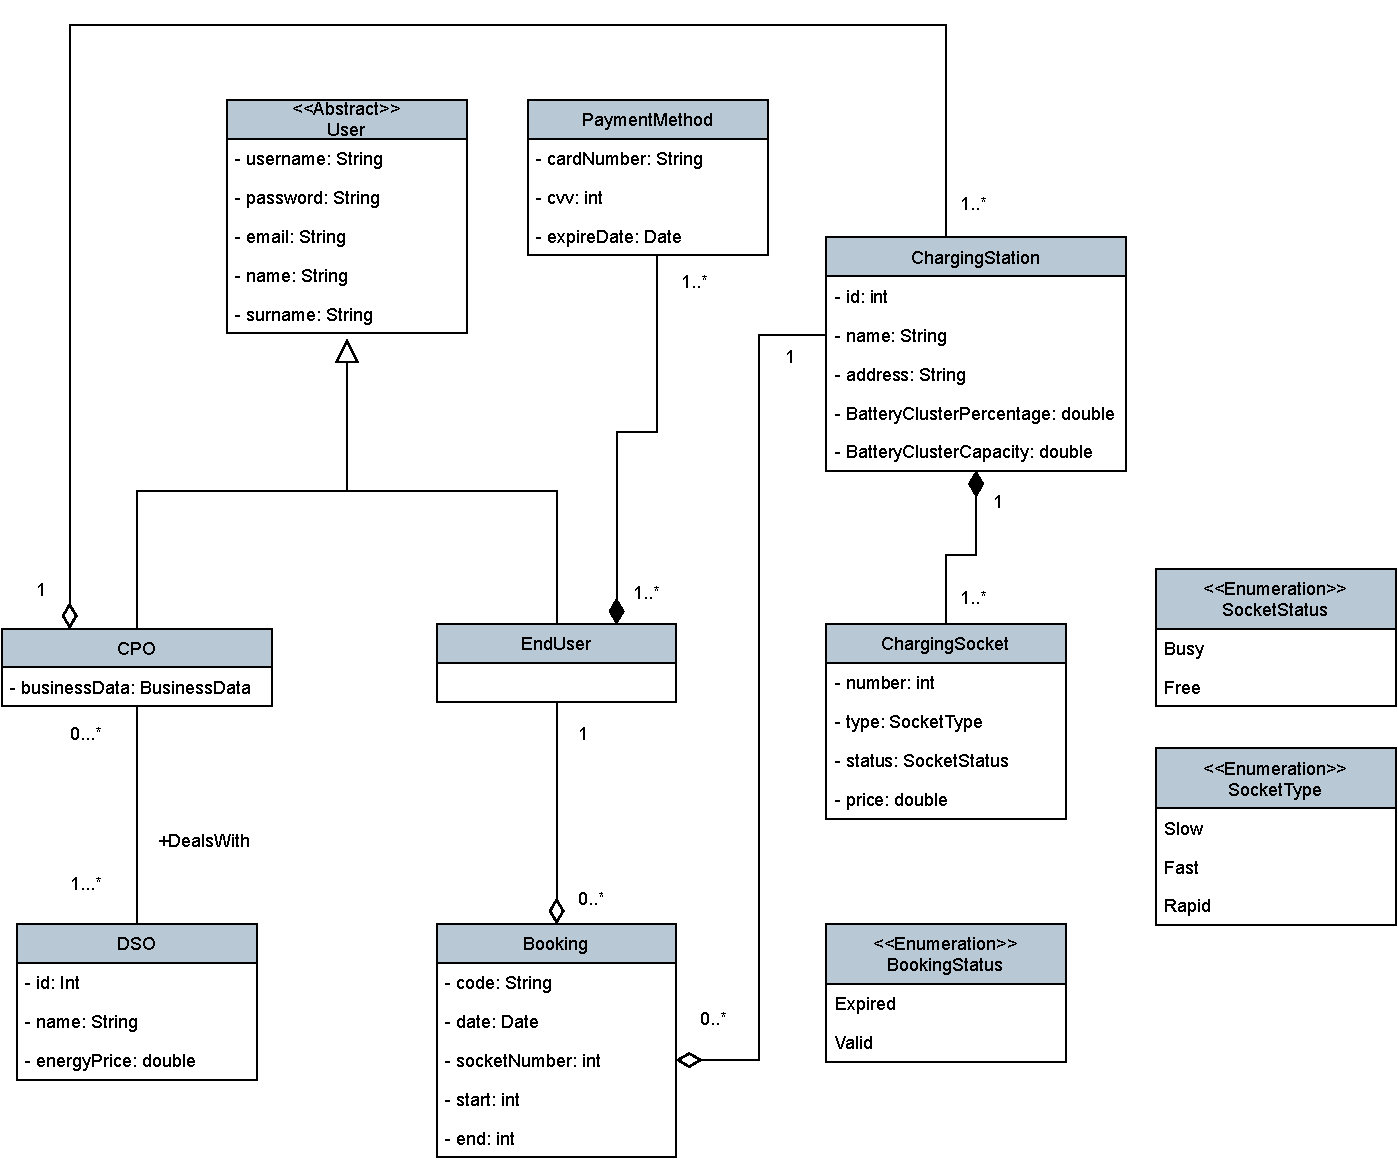
\includegraphics[width=0.9\textwidth]{images/classdiagram.pdf}
\caption{Class diagram}
\label{fig:class_diagram}
\end{center}
\end{figure}
\subsection{State diagram}
State diagrams model the behavior of a single object and are used for objects with significant dynamic behavior; they also specify the sequence of states that an object goes through during its lifetime in response to stimuli from the environment. In particular, they show the life history of a given class, the events that cause a transition from one state to another and the actions that result from a state change.\\
In this section we will represent the main state diagrams of the whole system.
\subsubsection{Authentication}
In figure \ref{fig:authentication} the authentication process carried out by both end users and the CPO is highlighted. First of all, the user (CPO/end user) has the possibility to register: if registration fails the system will repeat the operation, while if successful the user can log in. \\
If the end user or the CPO previously had an account, then they can log in directly: if the username and password are correct, the system shows the dashboard relating to the role that the person attempting to access has, otherwise it asks to re-enter the credentials.\\
Figure \ref{fig:booking} shows how this procedure is used before the booking process, obviously by end users.
\begin{figure}[H]
\begin{center}
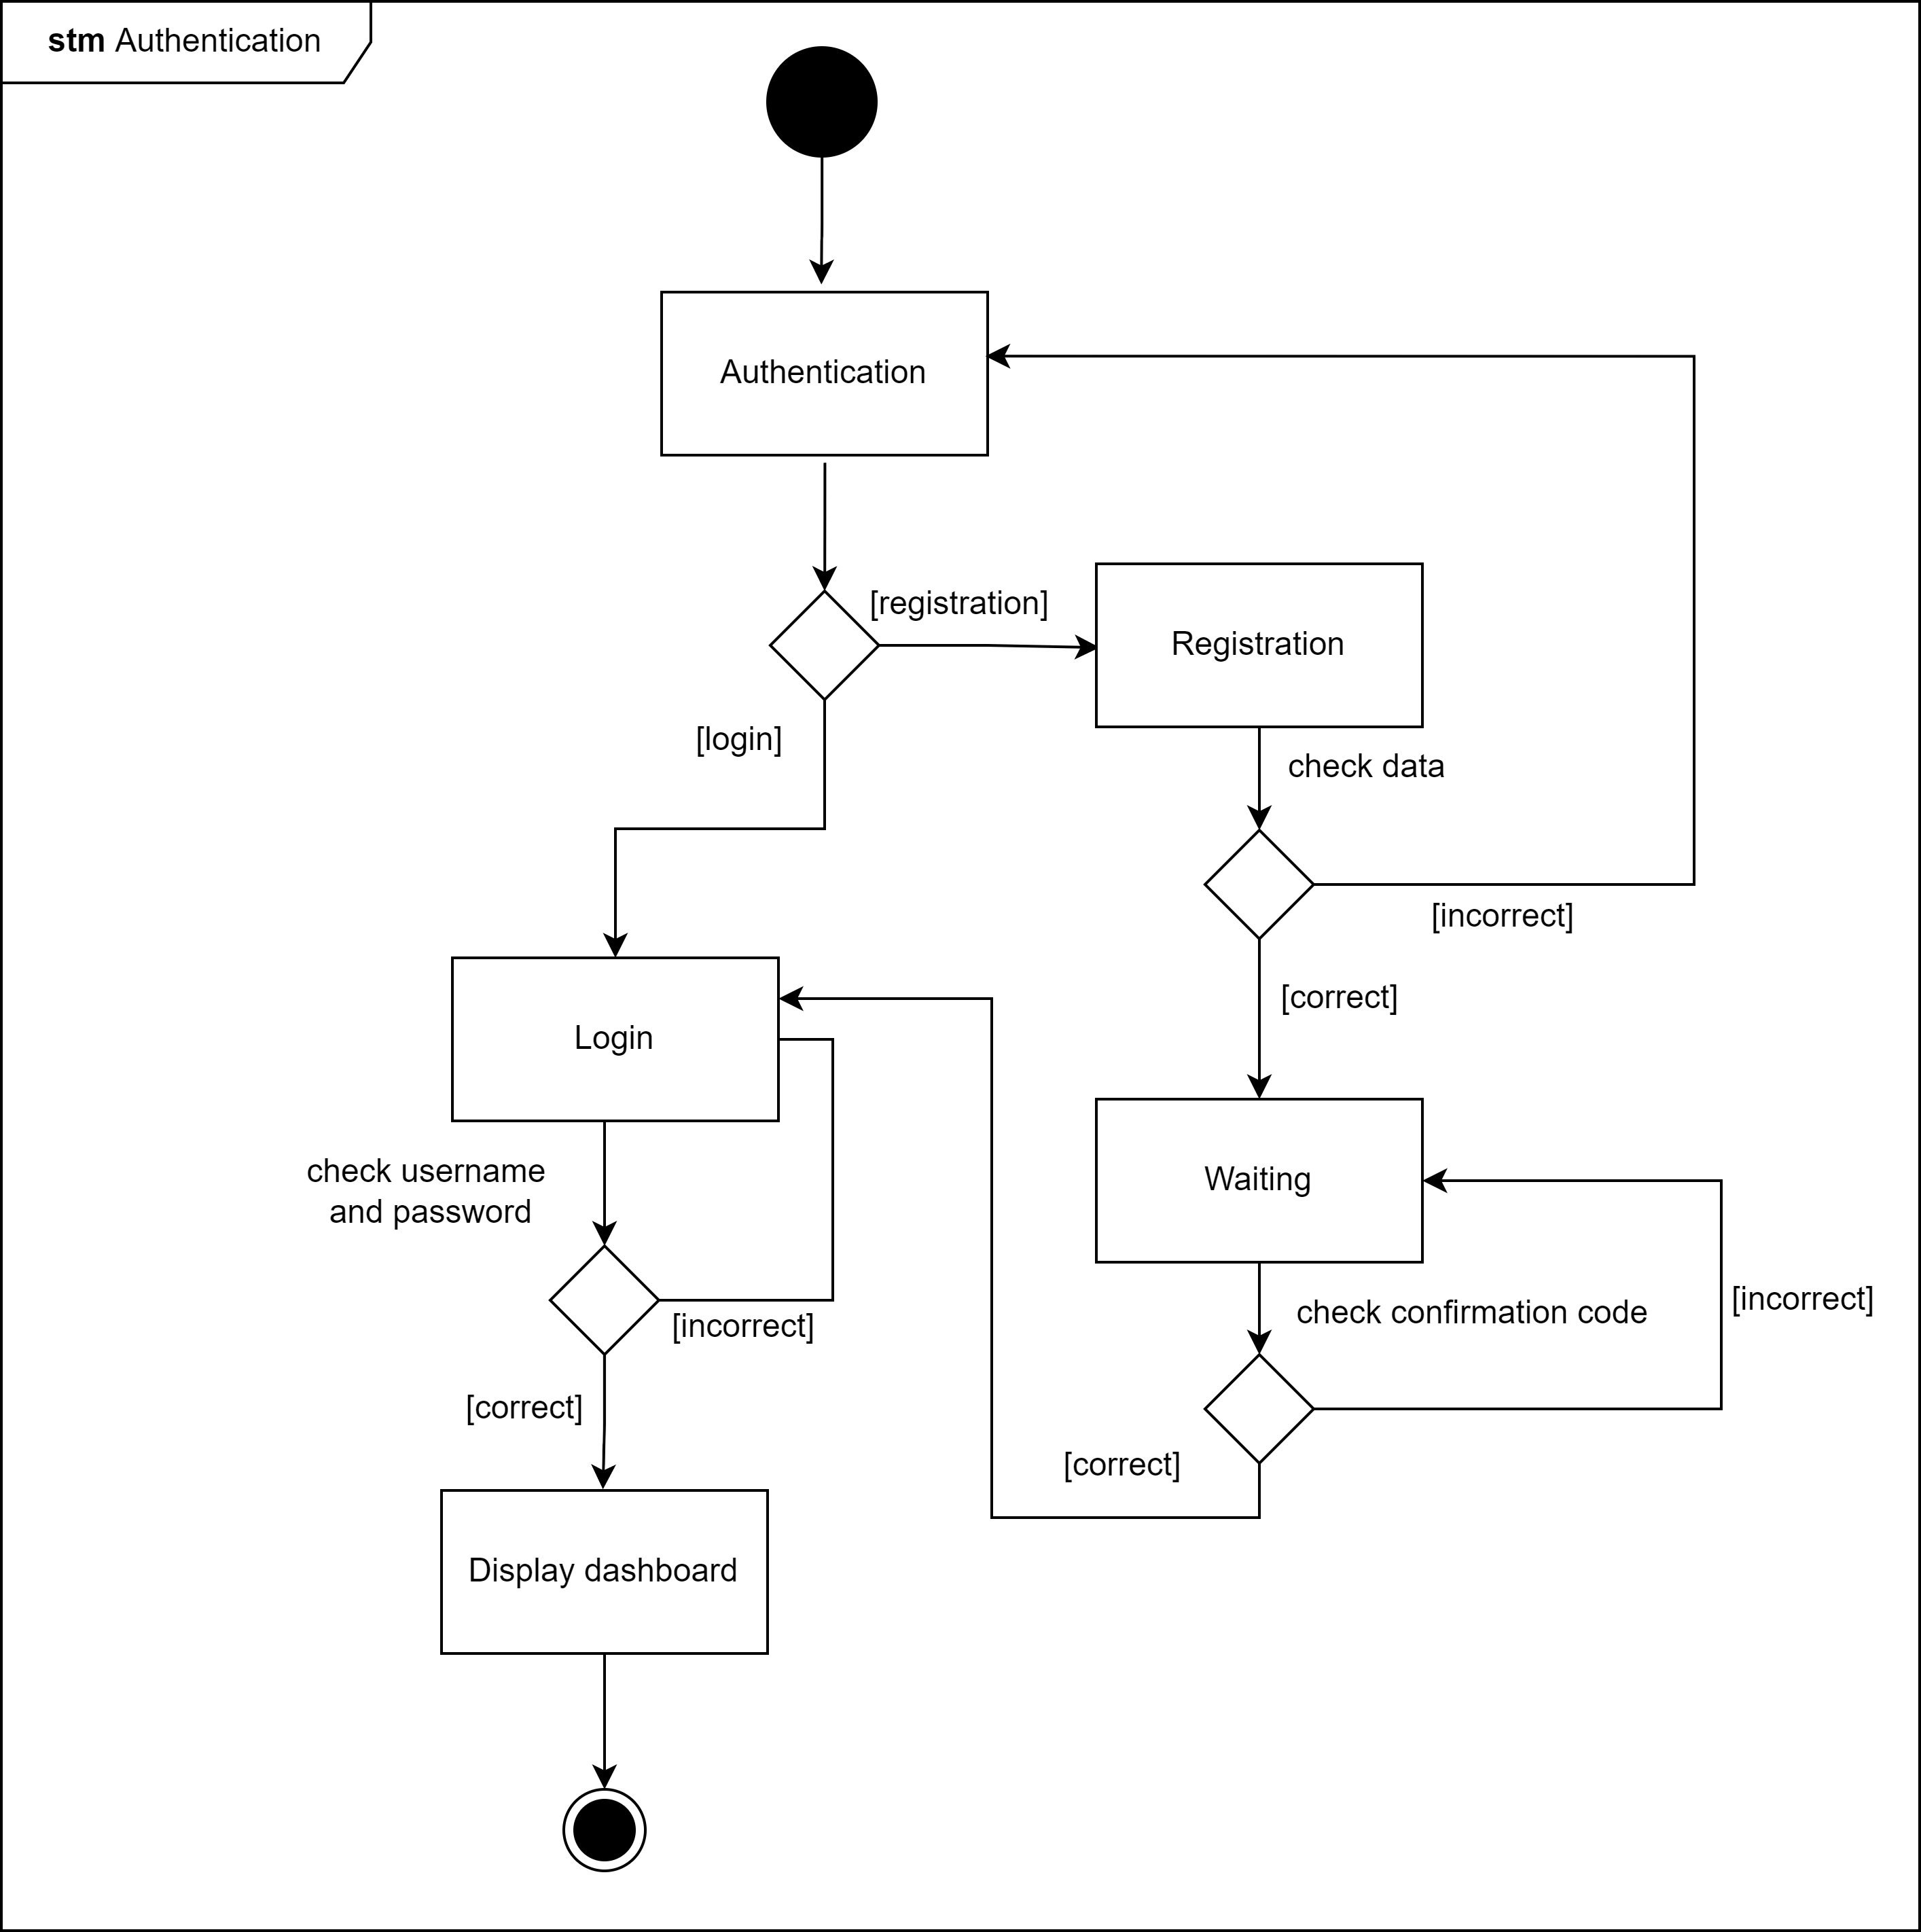
\includegraphics[width=0.7\textwidth]{images/authentication.png}
\caption{Authentication state diagram}
\label{fig:authentication}
\end{center}
\end{figure}
\subsubsection{Booking}
In the following figure is shown the process of reserving the charging socket by the end users. After logging in successfully, the reservation is created by choosing the preferred charging station, charging socket and timeframe: the system checks the validity of the choice and repeats the process if incorrect. If correct, a valid QR-Code is generated for the subsequent recognition of the user at the correct station (as explained in detail in figure \ref{fig:qr-code}). Obviously, after the reservation has been made successfully, the system also provides the possibility to delete it.
\begin{figure}[H]
\begin{center}
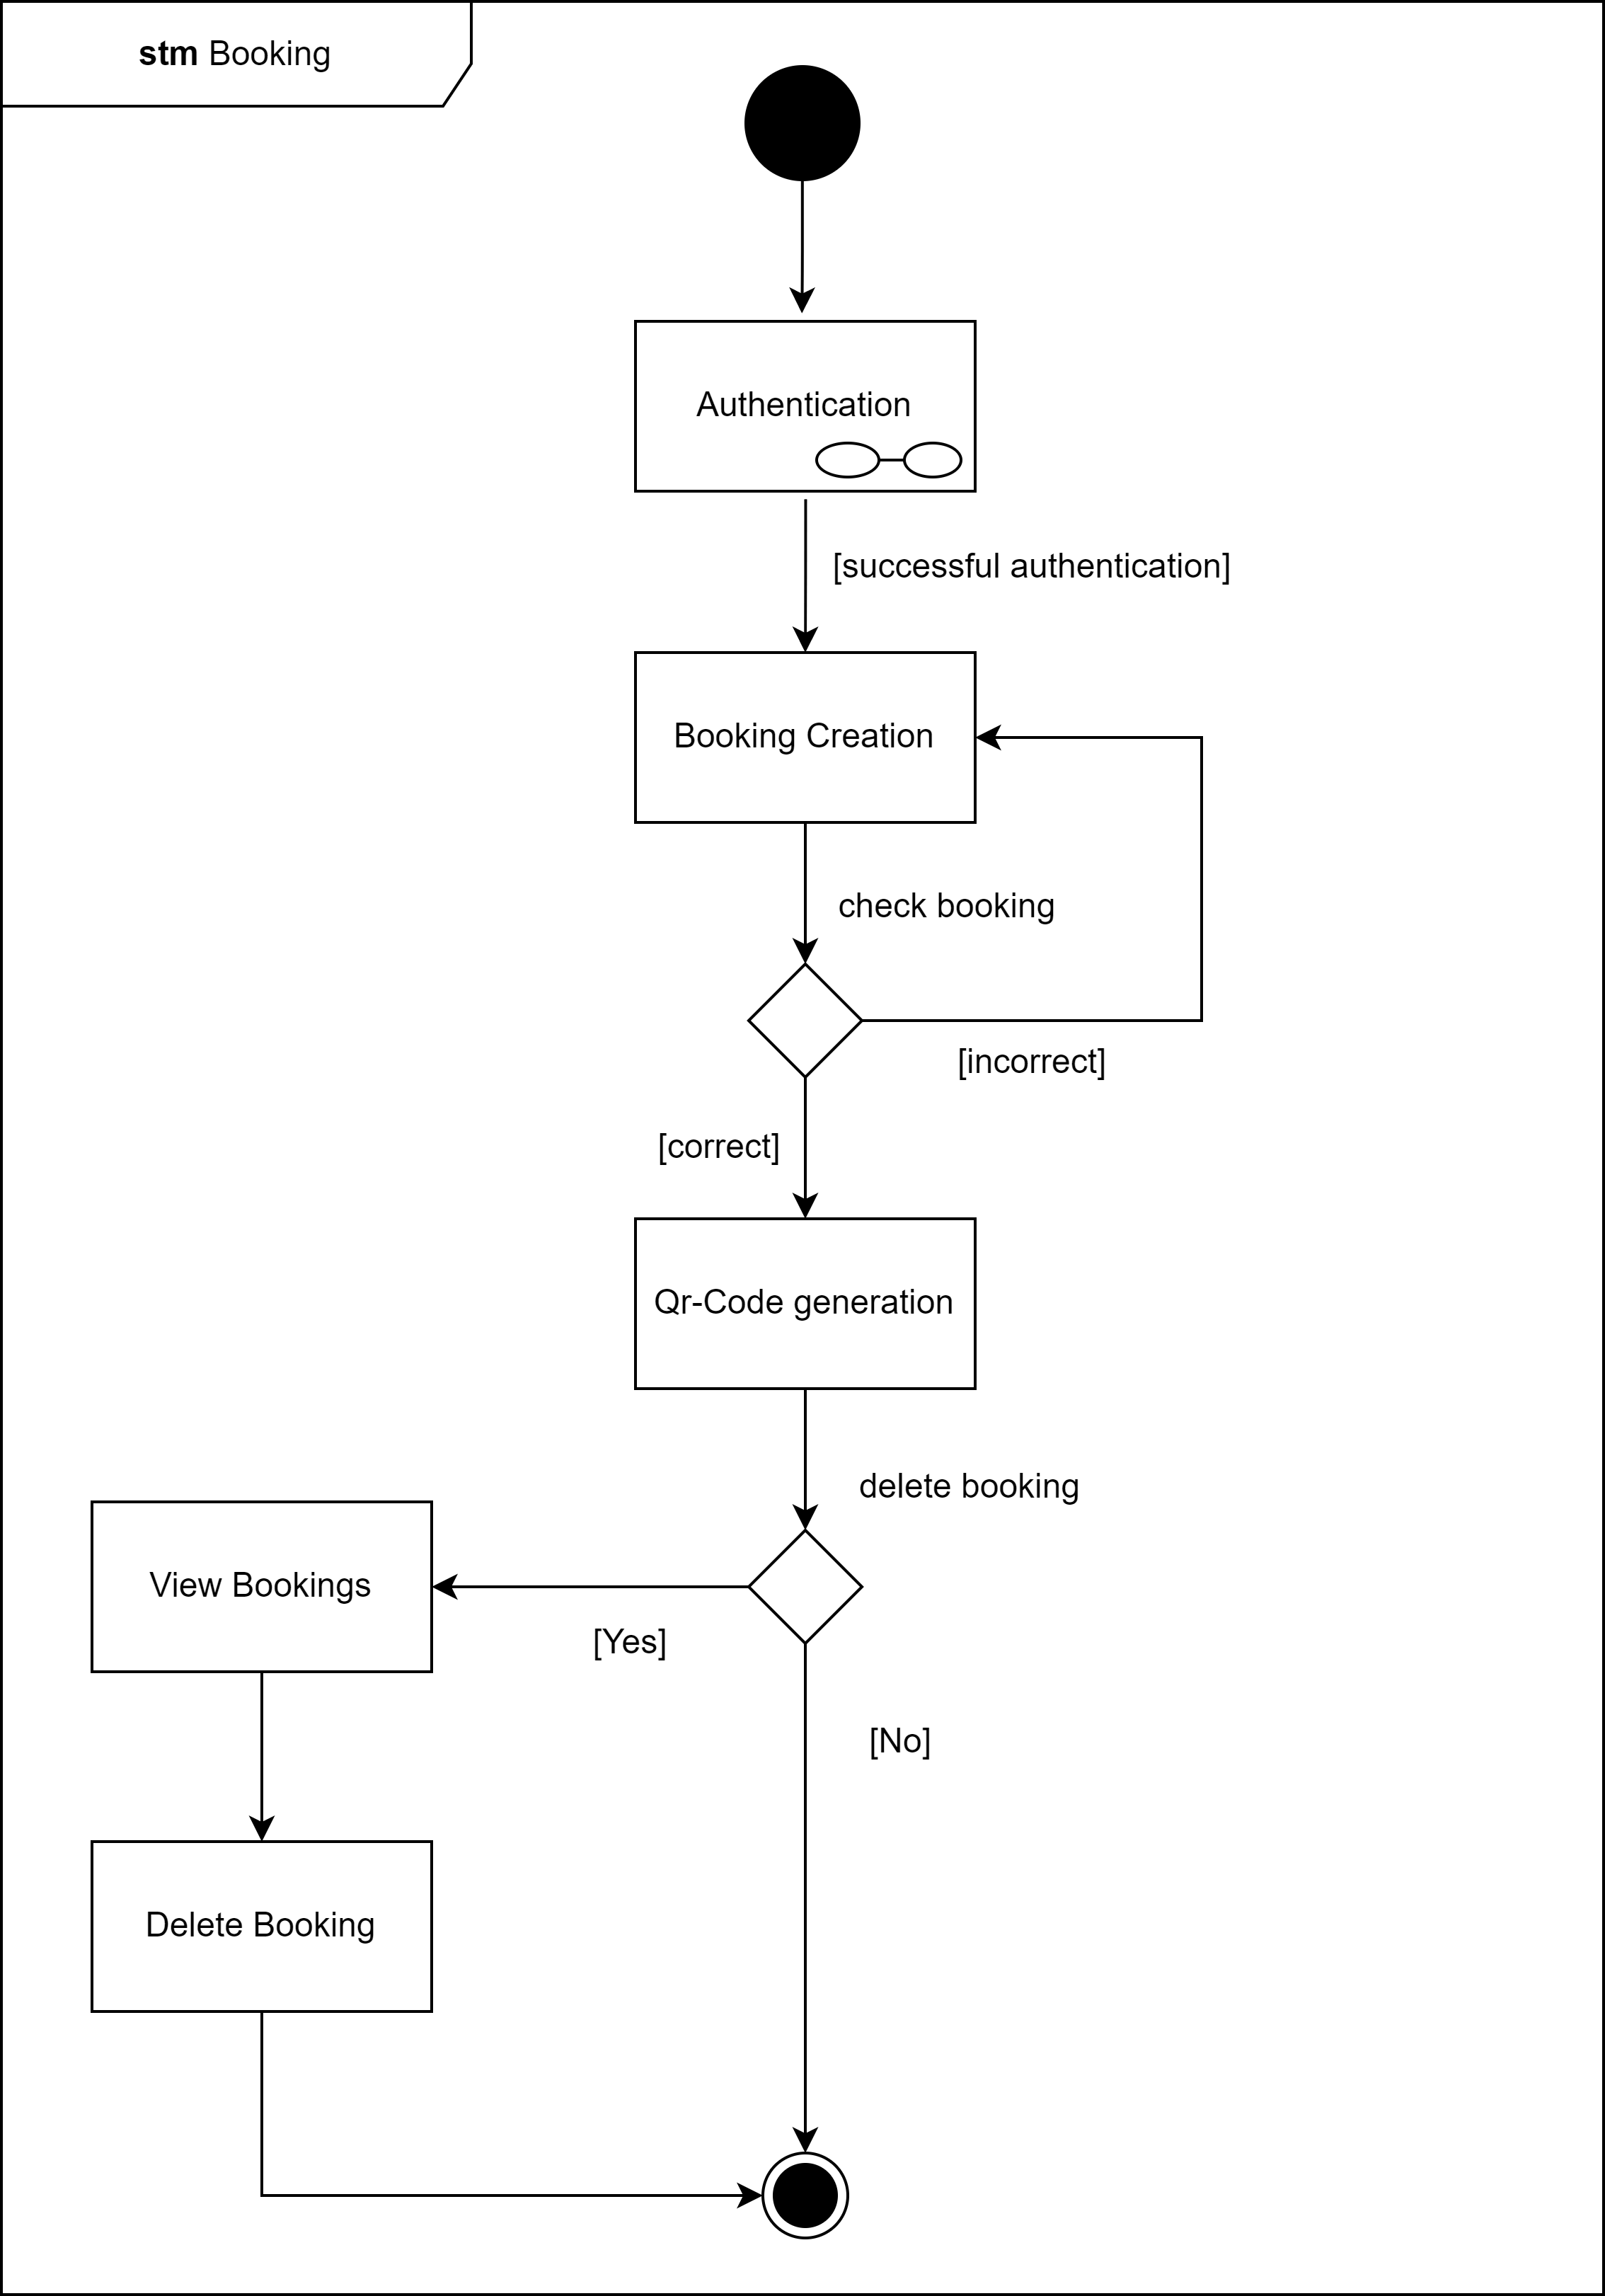
\includegraphics[width=0.8\textwidth]{images/booking.png}
\caption{Booking state diagram}
\label{fig:booking}
\end{center}
\end{figure}
\clearpage
\subsubsection{QR-Code Recognition}
Figure \ref{fig:qr-code} shows how end users reservations are recognized by a charging socket of a specific charging station. First, the QR-Code is scanned from the smartphone and the system checks its existence; if it exists, its validity is checked in terms of expiration. If it has not expired, end users are allowed to charge their vehicle.
\begin{figure}[H]
\begin{center}
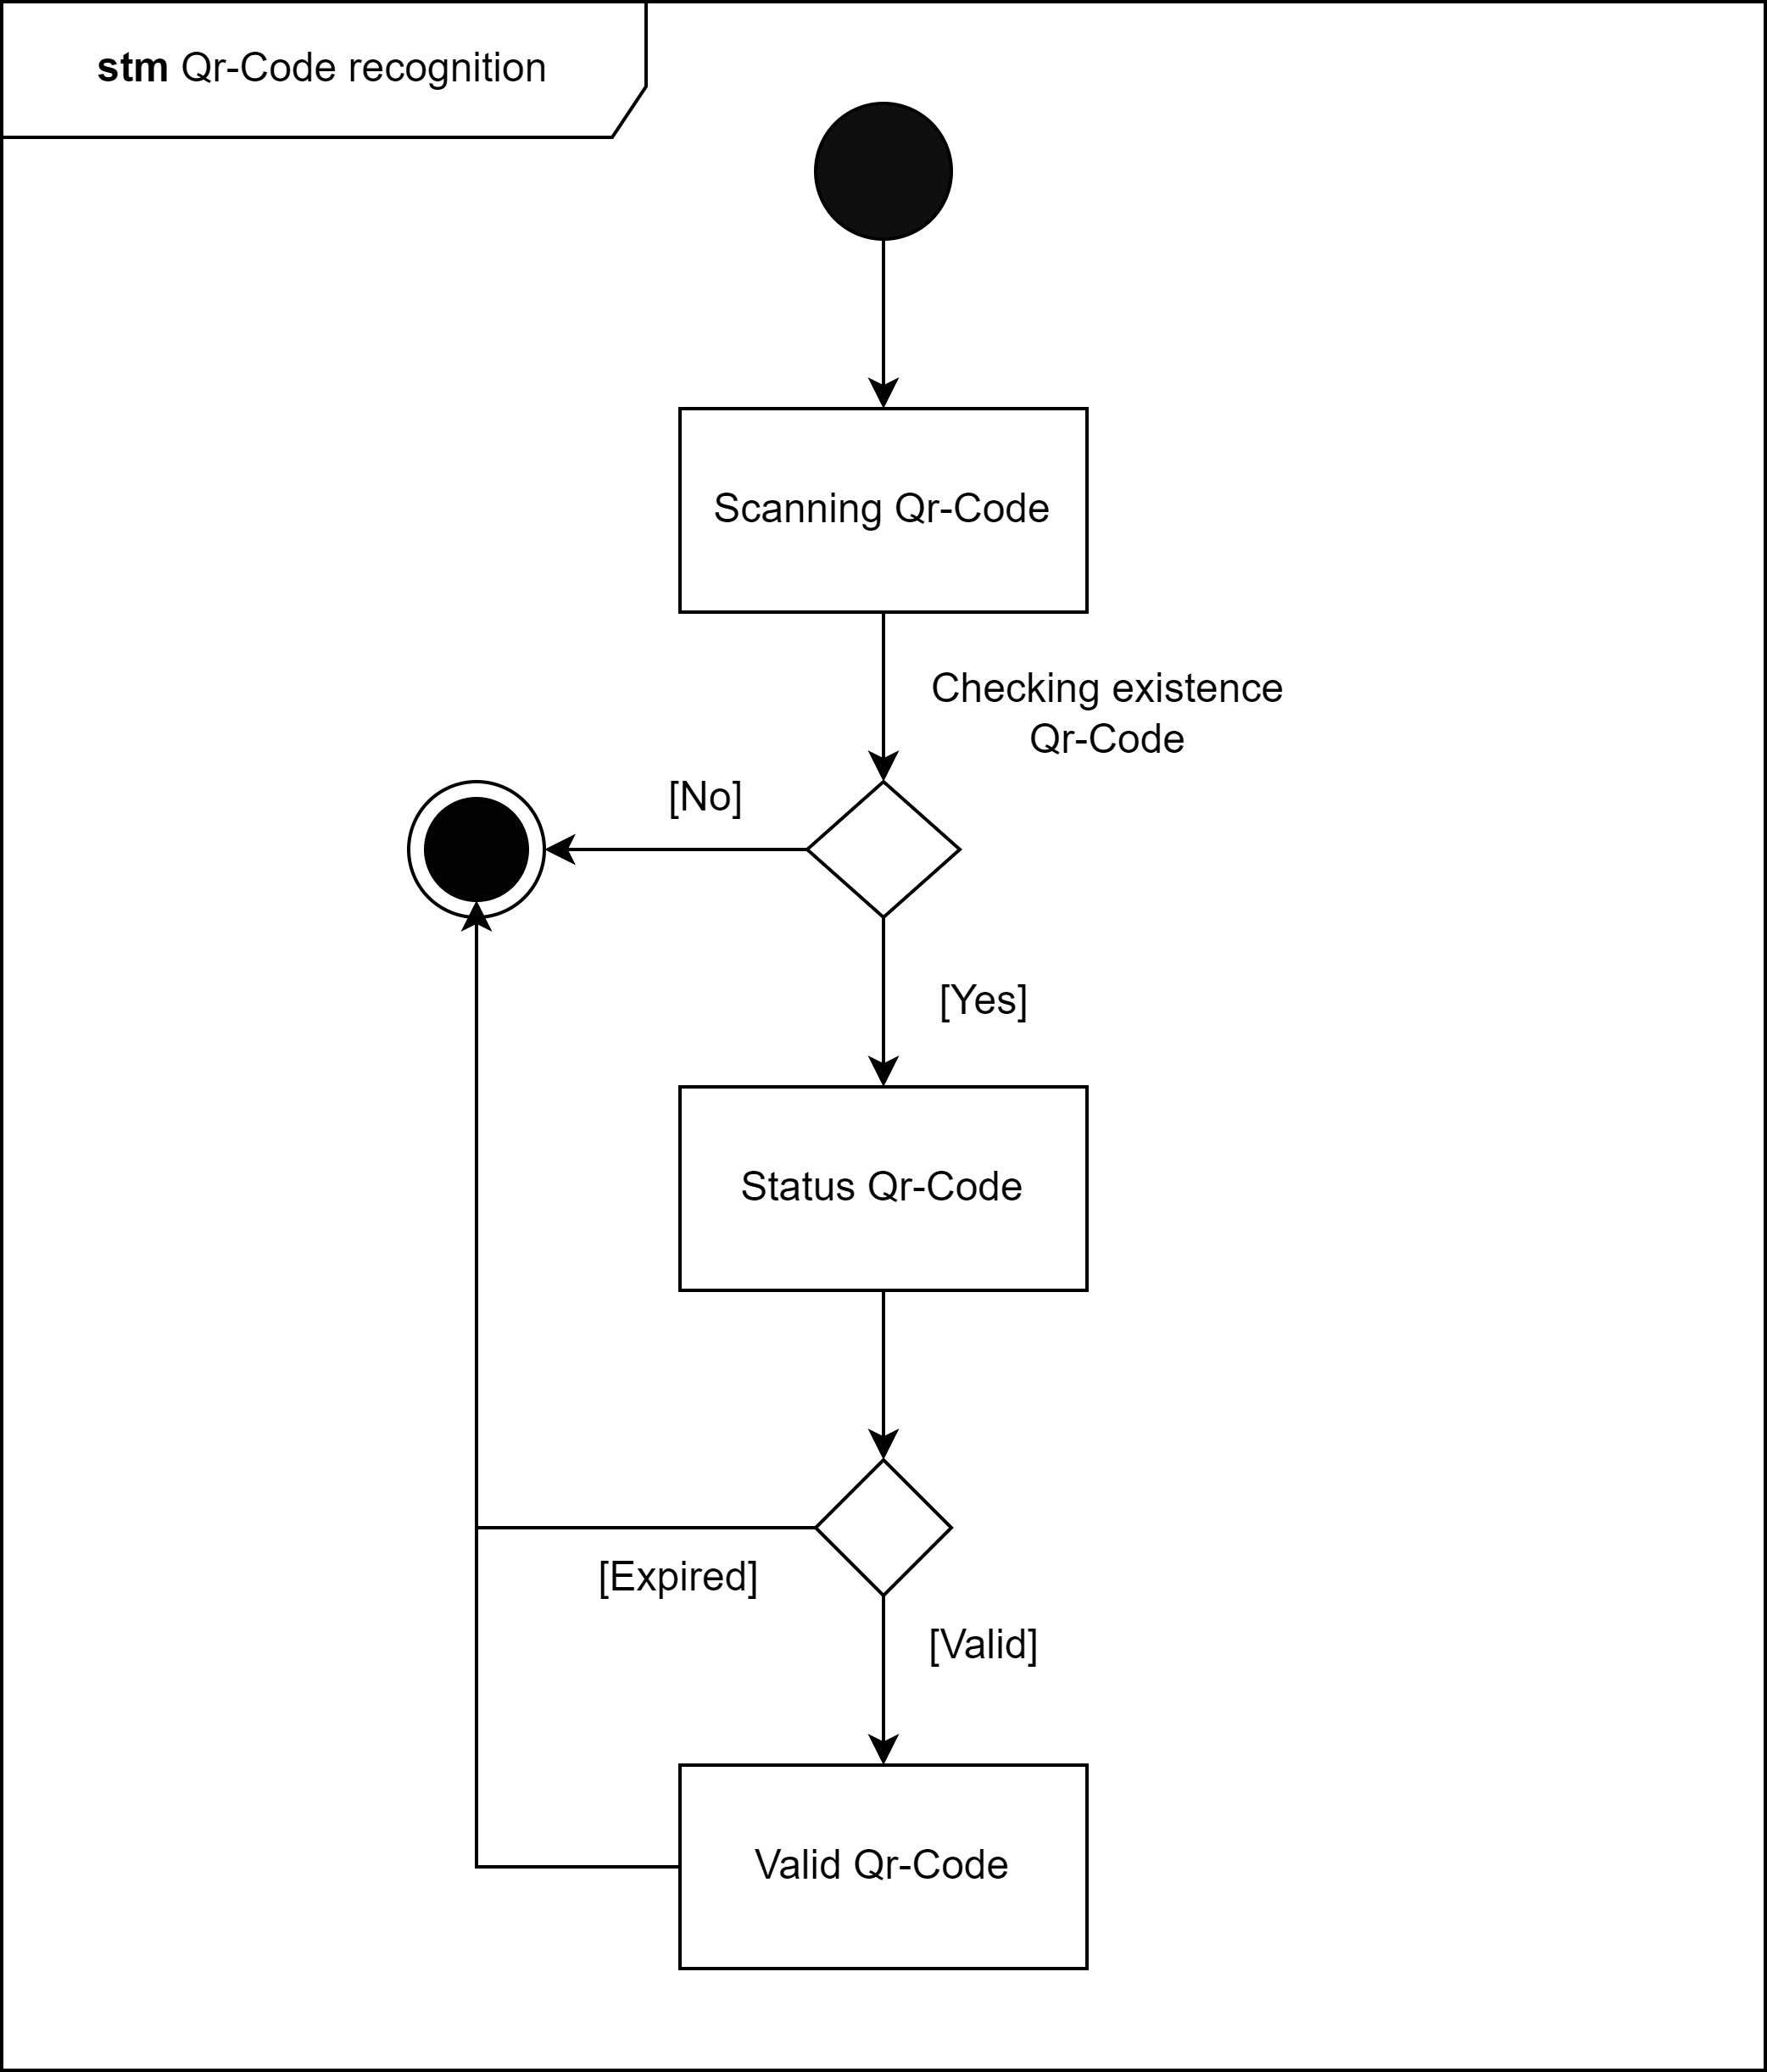
\includegraphics[width=1.0\textwidth]{images/qrcode.png}
\caption{Qr-Code Recognition state diagram}
\label{fig:qr-code}
\end{center}
\end{figure}

\section{Product functions}
In this section is presented a detailed description for each functionality that the platform provides, w.r.t the goals described in the first section \ref{sec:goals}.
\subsection{System authentication function}
The system allows both the end users and CPO to register an account and consequently login with that, but the two operations differ on the data which are provided during the registration. Obviously the privileges that a CPO and an end user have are completely different. 
\subsubsection{End users authentication}
End users have the possibility to log into the application using \textbf{username and password}. For the registration a new end user needs to provide username, password, an \textbf{email} and personal data. The email provided will be confirmed through a \textbf{OTP} received on the latter.
\subsubsection{CPOs authentication}
CPOs, like end users, have the possibility to log in into the application with \textbf{username and password}. The operation that is different from end users is the registration, in fact, a CPO in the registration phase must provide personal data, an  \textbf{email} but also \textbf{business data} related to the CPO's company. When a CPO is creating a new account he also needs to provide information related to his charging station. The email provided will be confirmed through a \textbf{OTP} received on the latter.
\subsection{Charging station booking function}
A reservation specifies three main points of information, that are:
\begin{itemize}
    \item The designated charging station.
    \item A charging socket installed in the station.
    \item A time interval in which the end user will charge his vehicle. 
\end{itemize}
Obviously the reservations can't overlap each other, an end user in fact can't book a charge in two different stations at the same time, but he can book multiple charges in different days for examples. The eMSP also provides the possibility to \textbf{delete} a reservation if needed.
\subsubsection{Charging station search function}
The eMSP suggests to the end user the best options he has when he needs to charge his vehicle according to his calendar, the remaining amount of energy, the distance, the energy price, special offers available and more. Once the end user selects the most suitable station, the application, that deals with the end user GPS, sets up the navigation to the charging point.
\subsubsection{Booking confirmation function}
When a customer makes a reservation a \textbf{QR-Code} is generated. The code is important because it represents in a \textbf{unique way} the reservation and is mandatory to verify the identity of the customer at the charging point, avoiding scams and to assure the correct usage of the charging sockets.
\subsubsection{Booking validation function}
When an end user reaches the designated charging station and consequently the assigned socket, he needs to confirm to the system that he actually made the reservation. To do so the end user uses the proper \textbf{QR-Code scanner} on the socket, which deals with the validation process and allows the charging operation. A reservation is valid until the upper bound of the time slot \textbf{is past}: in this case the user isn't allowed to charge his vehicle and needs to book again.
\subsubsection{Booking payment function}
Once the charging process is completed, the system will automatically subtract the correct amount of money from the \textbf{payment method} specified by the user on his account. After the payment the user will receive an \textbf{invoice} on his personal (confirmed) email.
\subsection{Charging station management function}
The CPMS supplies functionalities that are used by various CPOs to manage their stations: the functions vary from the charging socket interaction to the dialogue with the DSO.
\subsubsection{Energy acquisition function}
The CPMS provides to the CPO the possibility to \textbf{dinamically buy energy} from third parties distributors (DSO). For "dinamically buy" is intended that the purchase is made considering different aspects like the comparison between energy prices of multiple DSOs.  
\subsubsection{Energy distribution function}
Through the CPMS's dashboard, the CPO can decide the energy selling price and can also set special offers for his end users. The selling price and, consequently, the offers depend on the purchase price and on the energy source. The possible energy sources are storage batteries or the direct links with the DSO. The choice of the energy supply, for charging vehicles, can be automatically made by the CPMS or manually by the CPO with the aim of saving money w.r.t. the scenario described in \ref{sec:explsaving} and to reduce the energy impact on electric network, paying particular attention to avoid absorption peaks.
\subsubsection{Station monitoring function}
Using the CPMS, the CPO can monitor both internal and external status. For internal status are intended the following features: 
\begin{itemize}
    \item Level of energy in its batteries.
    \item Number of vehicles being charged.
    \item Amount of power absorbed for each charging vehicle.
    \item Time left to the end of the charge.
\end{itemize}
While for external status are intended the following points:
\begin{itemize}
    \item Number of charging sockets available.
    \item The socket type (slow/fast/rapid) .
    \item The socket cost.
    \item The estimated amount of time until the first socket of a type is freed.
\end{itemize}
\subsubsection{Charging termination function}
The system automatically notifies the user when the charging operation of his vehicle ends.
\subsubsection{New infrastructure function}
The CPO is able to add a new charging station and a new charging socket to the system, providing various information like: the position, the organization etc.
\section{User characteristics}
The eMall system has two user categories:
\begin{itemize}
    \item \textbf{End users}: they are the main users of the system who use the eMSP, and they can be of two types: 
    \begin{itemize}
        \item driving license holders
        \item non-holders
    \end{itemize}
    The latter may want to use the system to help or advise relatives and/or friends or, more simply, for pure personal interest.
    \item \textbf{CPOs}: The CPOs are administrators and owners of various charging stations. They also have to provide, when necessary, all the commercial information. \\
    They are able to manage the station in all its aspects, also purchasing energy from third parties (DSO). Although the application is simple to use, it is assumed that they have taken the online course for CPO.
\end{itemize}
\clearpage
\section{Assumptions, dependencies and constraints}
\subsection{Assumptions and Dependencies}
The assumptions, in the domain of interest of eMall, are illustrated below:

\begin{longtable}{|c|l|}
\hline
\rowcolor[HTML]{B8C8D5} 
{\color[HTML]{000000} \textbf{Assumptions}} & \multicolumn{1}{c|}{\cellcolor[HTML]{B8C8D5}{\color[HTML]{000000} \textbf{Description}}} \\ \hline
\endfirsthead
%
\endhead
D.1 \label{D.1}& \begin{tabular}[c]{@{}l@{}}All end users must have a smartphone with an available Internet\\ connection.\end{tabular} \\ \hline
D.2 \label{D.2}& All smartphones used must have a functioning and actionable GPS. \\ \hline
D.3 \label{D.3}& All end users must have at least one electric vehicle to charge. \\ \hline
D.4 \label{D.4}& All end users must give consent to the system to access their calendar. \\ \hline
D.5 \label{D.5}& \begin{tabular}[c]{@{}l@{}}All end users must give consent to the system to access their \\ navigation system and the status of battery of their vehicles.\end{tabular} \\ \hline
D.6 \label{D.6}& \begin{tabular}[c]{@{}l@{}}All charging stations have a QR-Code scanner that allows to recognize a\\ specific end user in a specif time slot.\end{tabular} \\ \hline
D.7 \label{D.7}& \begin{tabular}[c]{@{}l@{}}All end users must have a working charging cable and any adapters\\ useful for charging process.\end{tabular} \\ \hline
D.8 \label{D.8}& \begin{tabular}[c]{@{}l@{}}All end users must be able to link cable from stations to vehicles\\ and to charge vehicles themselves.\end{tabular} \\ \hline
D.9 \label{D.9}& All CPOs must have Internet connection to use CPMS software. \\ \hline
D.10 \label{D.10}& All CPOs must have the adeguate IT infrastructure. \\ \hline
D.11 \label{D.11}& \begin{tabular}[c]{@{}l@{}}All CPOs should have a good knowledge of the e-mobility domain.\end{tabular} \\ \hline
D.12 \label{D.12}& Charging stations have unique codes. \\ \hline
D.13 \label{D.13}& All CPOs have at least one charging station. \\ \hline
D.14 \label{D.14}& Qr-Codes are associated with a specific reservation. \\ \hline
D.15 \label{D.15}& \begin{tabular}[c]{@{}l@{}}All end users must have an email address to sign-up.\end{tabular} \\ \hline
D.16 \label{D.16}& \begin{tabular}[c]{@{}l@{}}All CPOs must have an email address and all commercial data \\ to sign-up.\end{tabular} \\ \hline
D.17 \label{D.17}& A timeslot begins and ends only at the hour on the dot.\\ \hline
D.18 \label{D.18}& Only end users start the charging process.\\ \hline
D.19 \label{D.19}& All charging stations are composed by at least one charging socket.\\ \hline
D.20 \label{D.20}& All charging sockets can charge one vehicle at a time.\\ \hline
D.21 \label{D.21}& A DSO has only one offer for the energy.\\ \hline
D.22 \label{D.22}& \begin{tabular}[c]{@{}l@{}}All charging sockets are "charging columns" with only one cable \\attachment.\end{tabular}\\ \hline
D.23 \label{D.23}&\begin{tabular}[c]{@{}l@{}} eMall doesn't handle the possible bankruptcy of a CPO or the closure\\ of a charging station.\end{tabular} \\ \hline
D.24 \label{D.24}&\begin{tabular}[c]{@{}l@{}} If the user does not have enough money to pay, if his bank does not allow\\ debt, the system will attempt to subtract the money periodically.\end{tabular} \\ \hline
D.25\label{D.25}& \begin{tabular}[c]{@{}l@{}}All CPOs don't have a payment method, as the billing of the energy\\ purchased by the DSOs is done externally to the eMall system.\end{tabular}\\ \hline
D.26 \label{D.26}& \begin{tabular}[c]{@{}l@{}}All end users have debit cards as a method of payment and cannot \\make bank transfers.\end{tabular}\\ \hline
D.27 \label{D.27}& \begin{tabular}[c]{@{}l@{}}All charging stations have a battery cluster to store the energy\\ purchased by the DSO.\end{tabular}\\ \hline
D.28 \label{D.28}& \begin{tabular}[c]{@{}l@{}}The name, the surname and the e-mail of the CPO are related to the representative \\ for the company which is in charge for the station monitor operations.\end{tabular}\\ \hline
D.29 \label{D.29}& \begin{tabular}[c]{@{}l@{}}For simplicity's sake, CPO business data is a company code of length\\ 10, that is unique in the whole system.\end{tabular}\\ \hline
D.30 \label{D.30}& \begin{tabular}[c]{@{}l@{}}Only one CPO per company exists.\end{tabular}\\ \hline
\end{longtable}
\subsection{Constraints}
In this section are illustrated limits and system features.
\subsubsection{Privacy policies}
The eMall system collects and uses the end user's and CPO's data to better manage the service provided. A user who wants to use the system must accept consent to the processing of data, which will not in any case be disclosed to third parties or used for marketing purposes.
\subsubsection{Hardware limitations}
Although eMall is a simple system to use, unfortunately it is not available on all devices. \\
The requirements that the devices exploiting the system must meet are listed below:
\begin{itemize}
    \item LTE/3G/4G/5G connection
    \item iPhone with iOS version at least 13.0
    \item Android with Android 6 Marshmallow
    \item GPS available
    \item Web Browser (Opera, Safari, Chrome, Firefox), for the CPO's app.
\end{itemize}
\subsubsection{Software limitations}
The system used is strictly related to the use of APIs regarding positioning on the map: they are necessary for the correct functioning of the platform. \\
Moreover, if the system does not have access to the user's calendar, battery status or navigation system, then eMall will not operate at its full capacity.